\documentclass[a4paper,12pt]{article}

\usepackage[utf8]{inputenc}
\usepackage[T1]{fontenc}
\usepackage[italian]{babel}
\usepackage{geometry}
\geometry{margin=2.5cm}
\usepackage{graphicx}
\usepackage{hyperref}
\usepackage{amsmath}
\usepackage{amssymb}
\usepackage{float}

\title{Relazione: Implementazione Protocollo Go-Back-N}
\author{Enrico Ancarani}
\date{\today}
\begin{document}
\maketitle
\tableofcontents
\newpage
\section{Descrizione del Sistema}
Il sistema implementa il protocollo Go-Back-N per la trasmissione di dati su UDP, composto da due componenti principali:
\begin{itemize}
    \item \textbf{Client (Trasmettitore)}: Invia pacchetti numerati sequenzialmente.
    \item \textbf{Server (Ricevitore)}: Riceve i pacchetti e invia acknowledgment (ACK).
\end{itemize}
\section{Funzionamento del Client}
\begin{itemize}
    \item \textbf{base}: primo pacchetto non ancora confermato.
    \item \textbf{next\_seq\_num}: prossimo numero di sequenza da inviare
\end{itemize}
\section{Logica di Invio}
\begin{itemize}
    \item Invia pacchetti fino al limite della finestra (\textbf{WINDOW\_SIZE} = 3)
    \item Simula perdite casuali con probabilità del 20\%
    \item Attende ACK per avanzare la finestra
    \item In caso di timeout, ritrasmette tutti i pacchetti dalla base della finestra
\end{itemize}
\section{Funzionamento del Server}
Il server mantiene:
\begin{itemize}
    \item \textbf{expectedPackageNumber}: numero di sequenza atteso
\end{itemize}
\section{Logica di Ricezione}
\begin{itemize}
    \item Accetta solo pacchetti con numero di sequenza corretto
    \item Per pacchetti corretti: invia ACK e incrementa il numero atteso
    \item Per pacchetti fuori ordine: invia ACK dell'ultimo pacchetto ricevuto correttamente
\end{itemize}
\section{Schema di Flusso - CLIENT}

\begin{figure}[H]
    \centering
    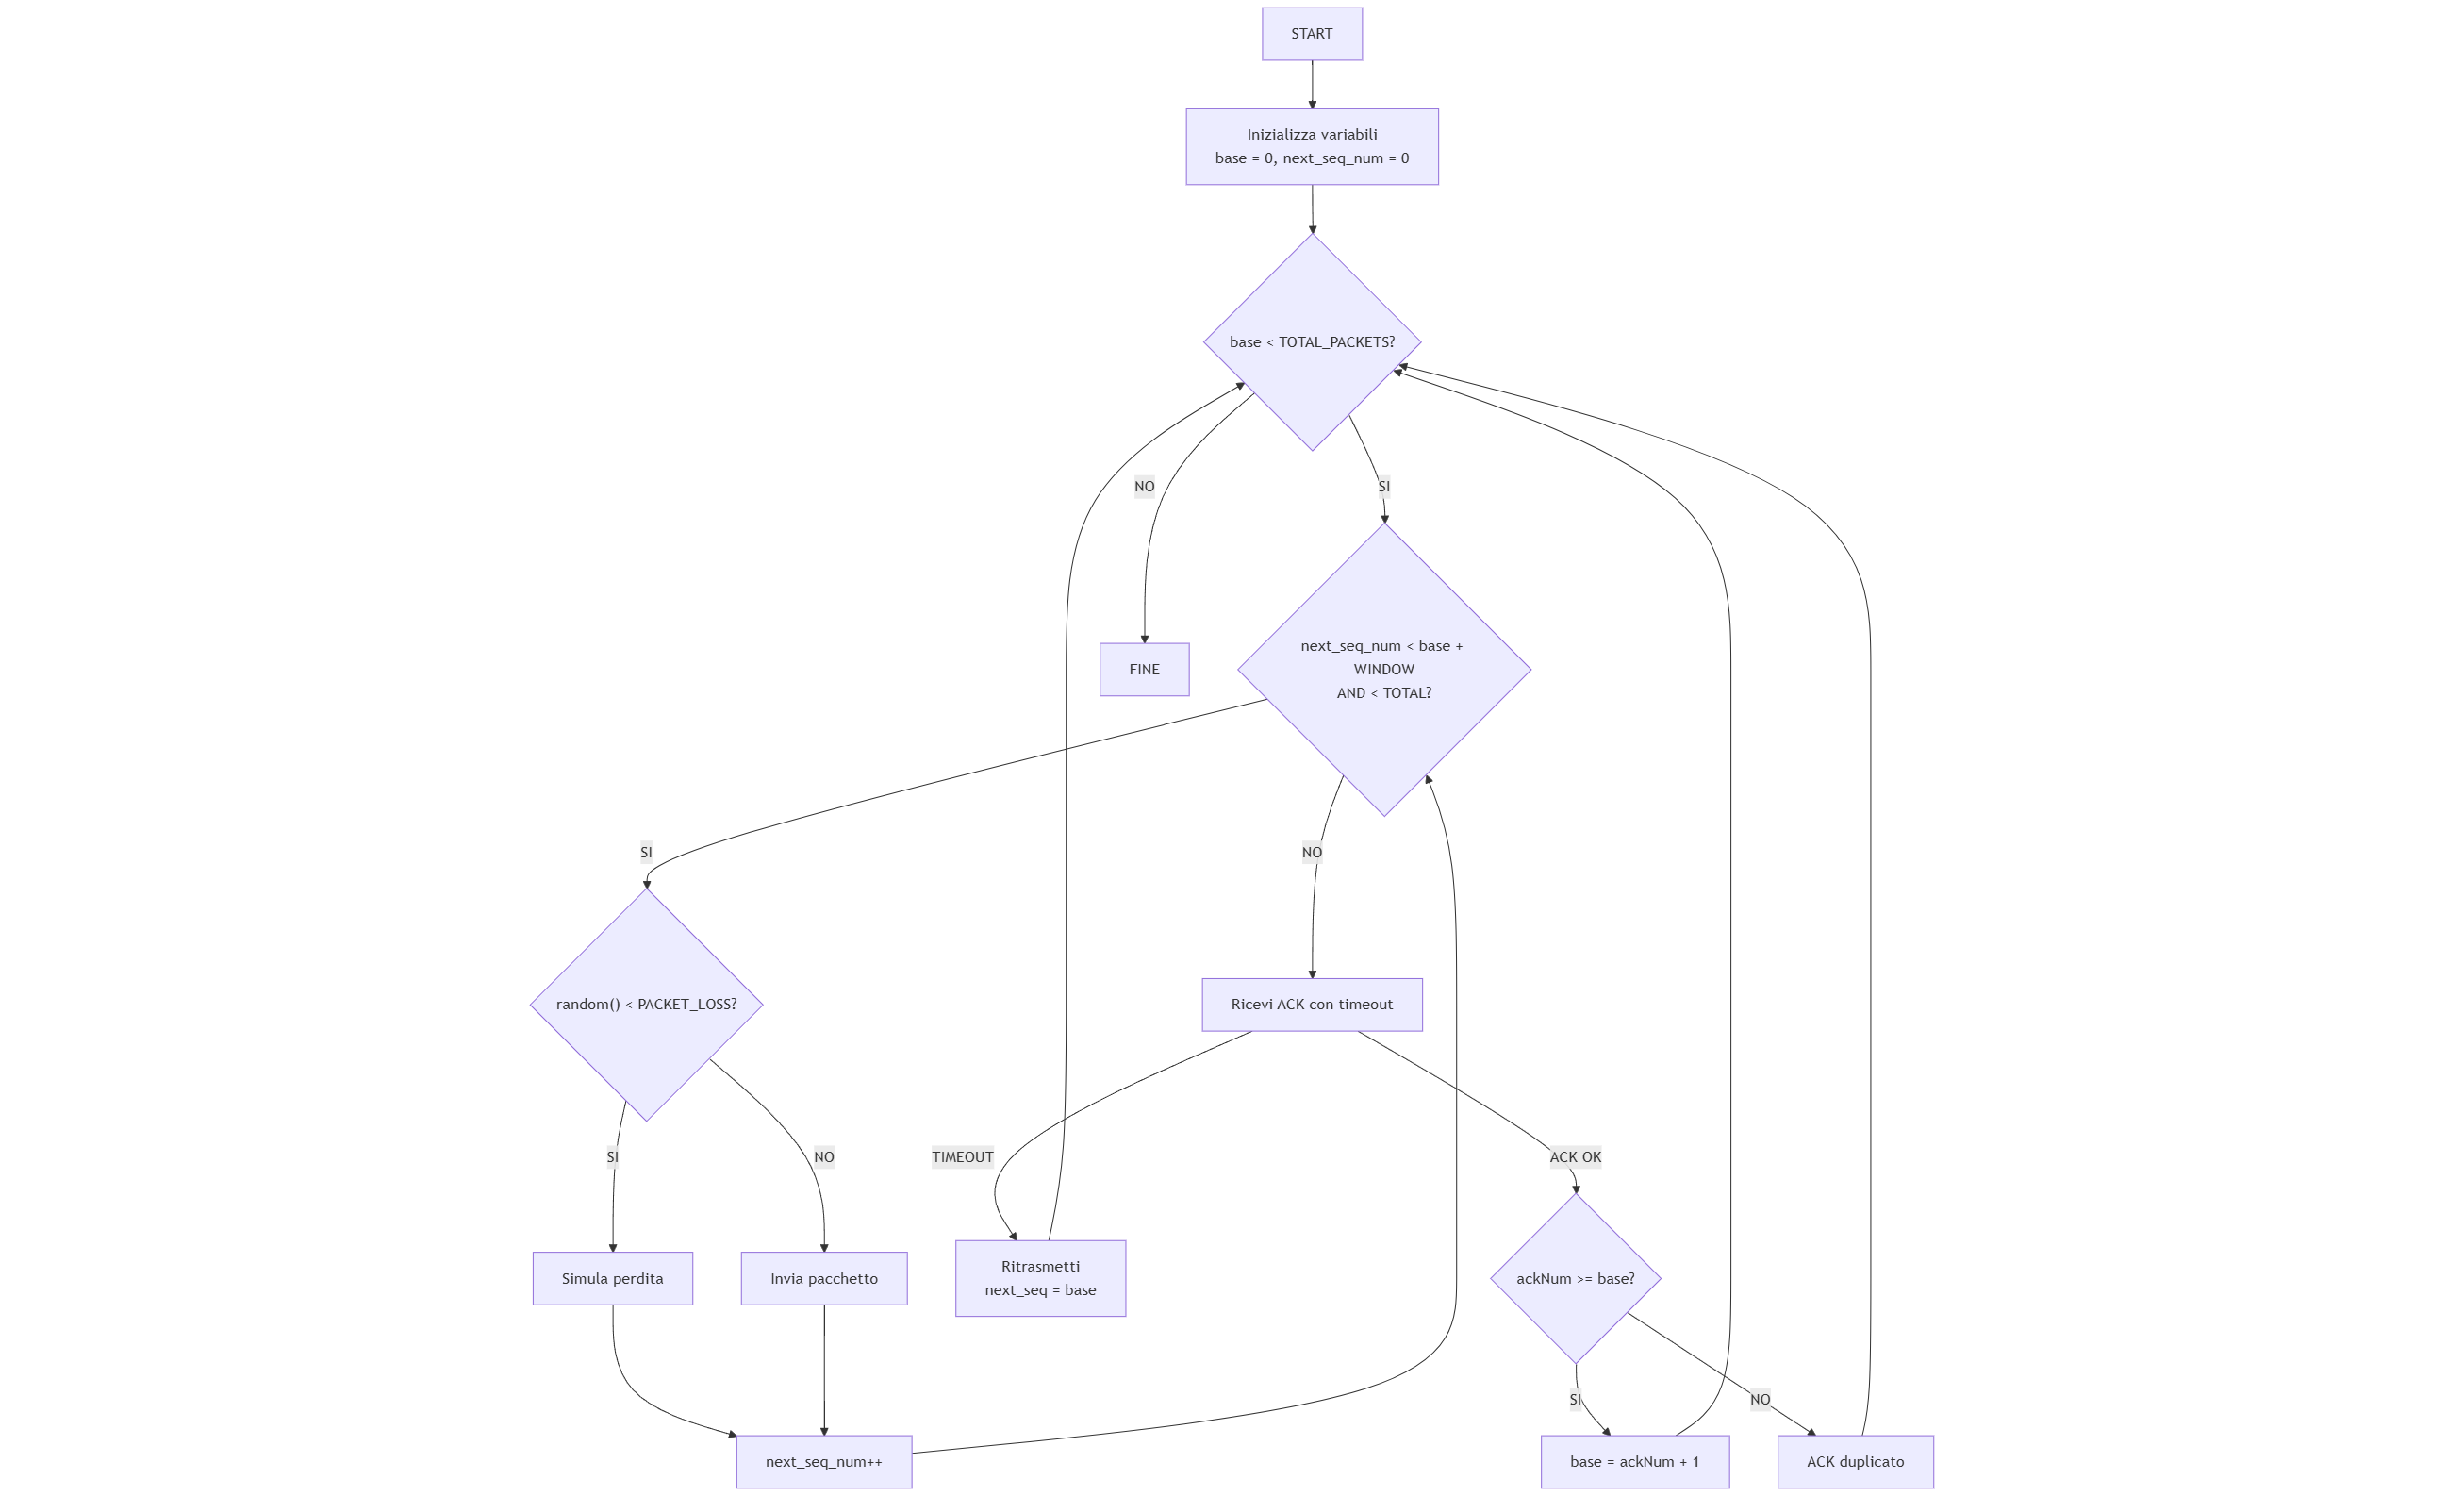
\includegraphics[width=\paperwidth, height=0.85\textheight, keepaspectratio]{img/SchemaDiFlussoClient.png}
    \caption{Schema di flusso del client}
    \label{img: schema di flusso del client}
\end{figure}
\section{Schema di Flusso - SERVER}

\begin{figure}[H]
    \centering
    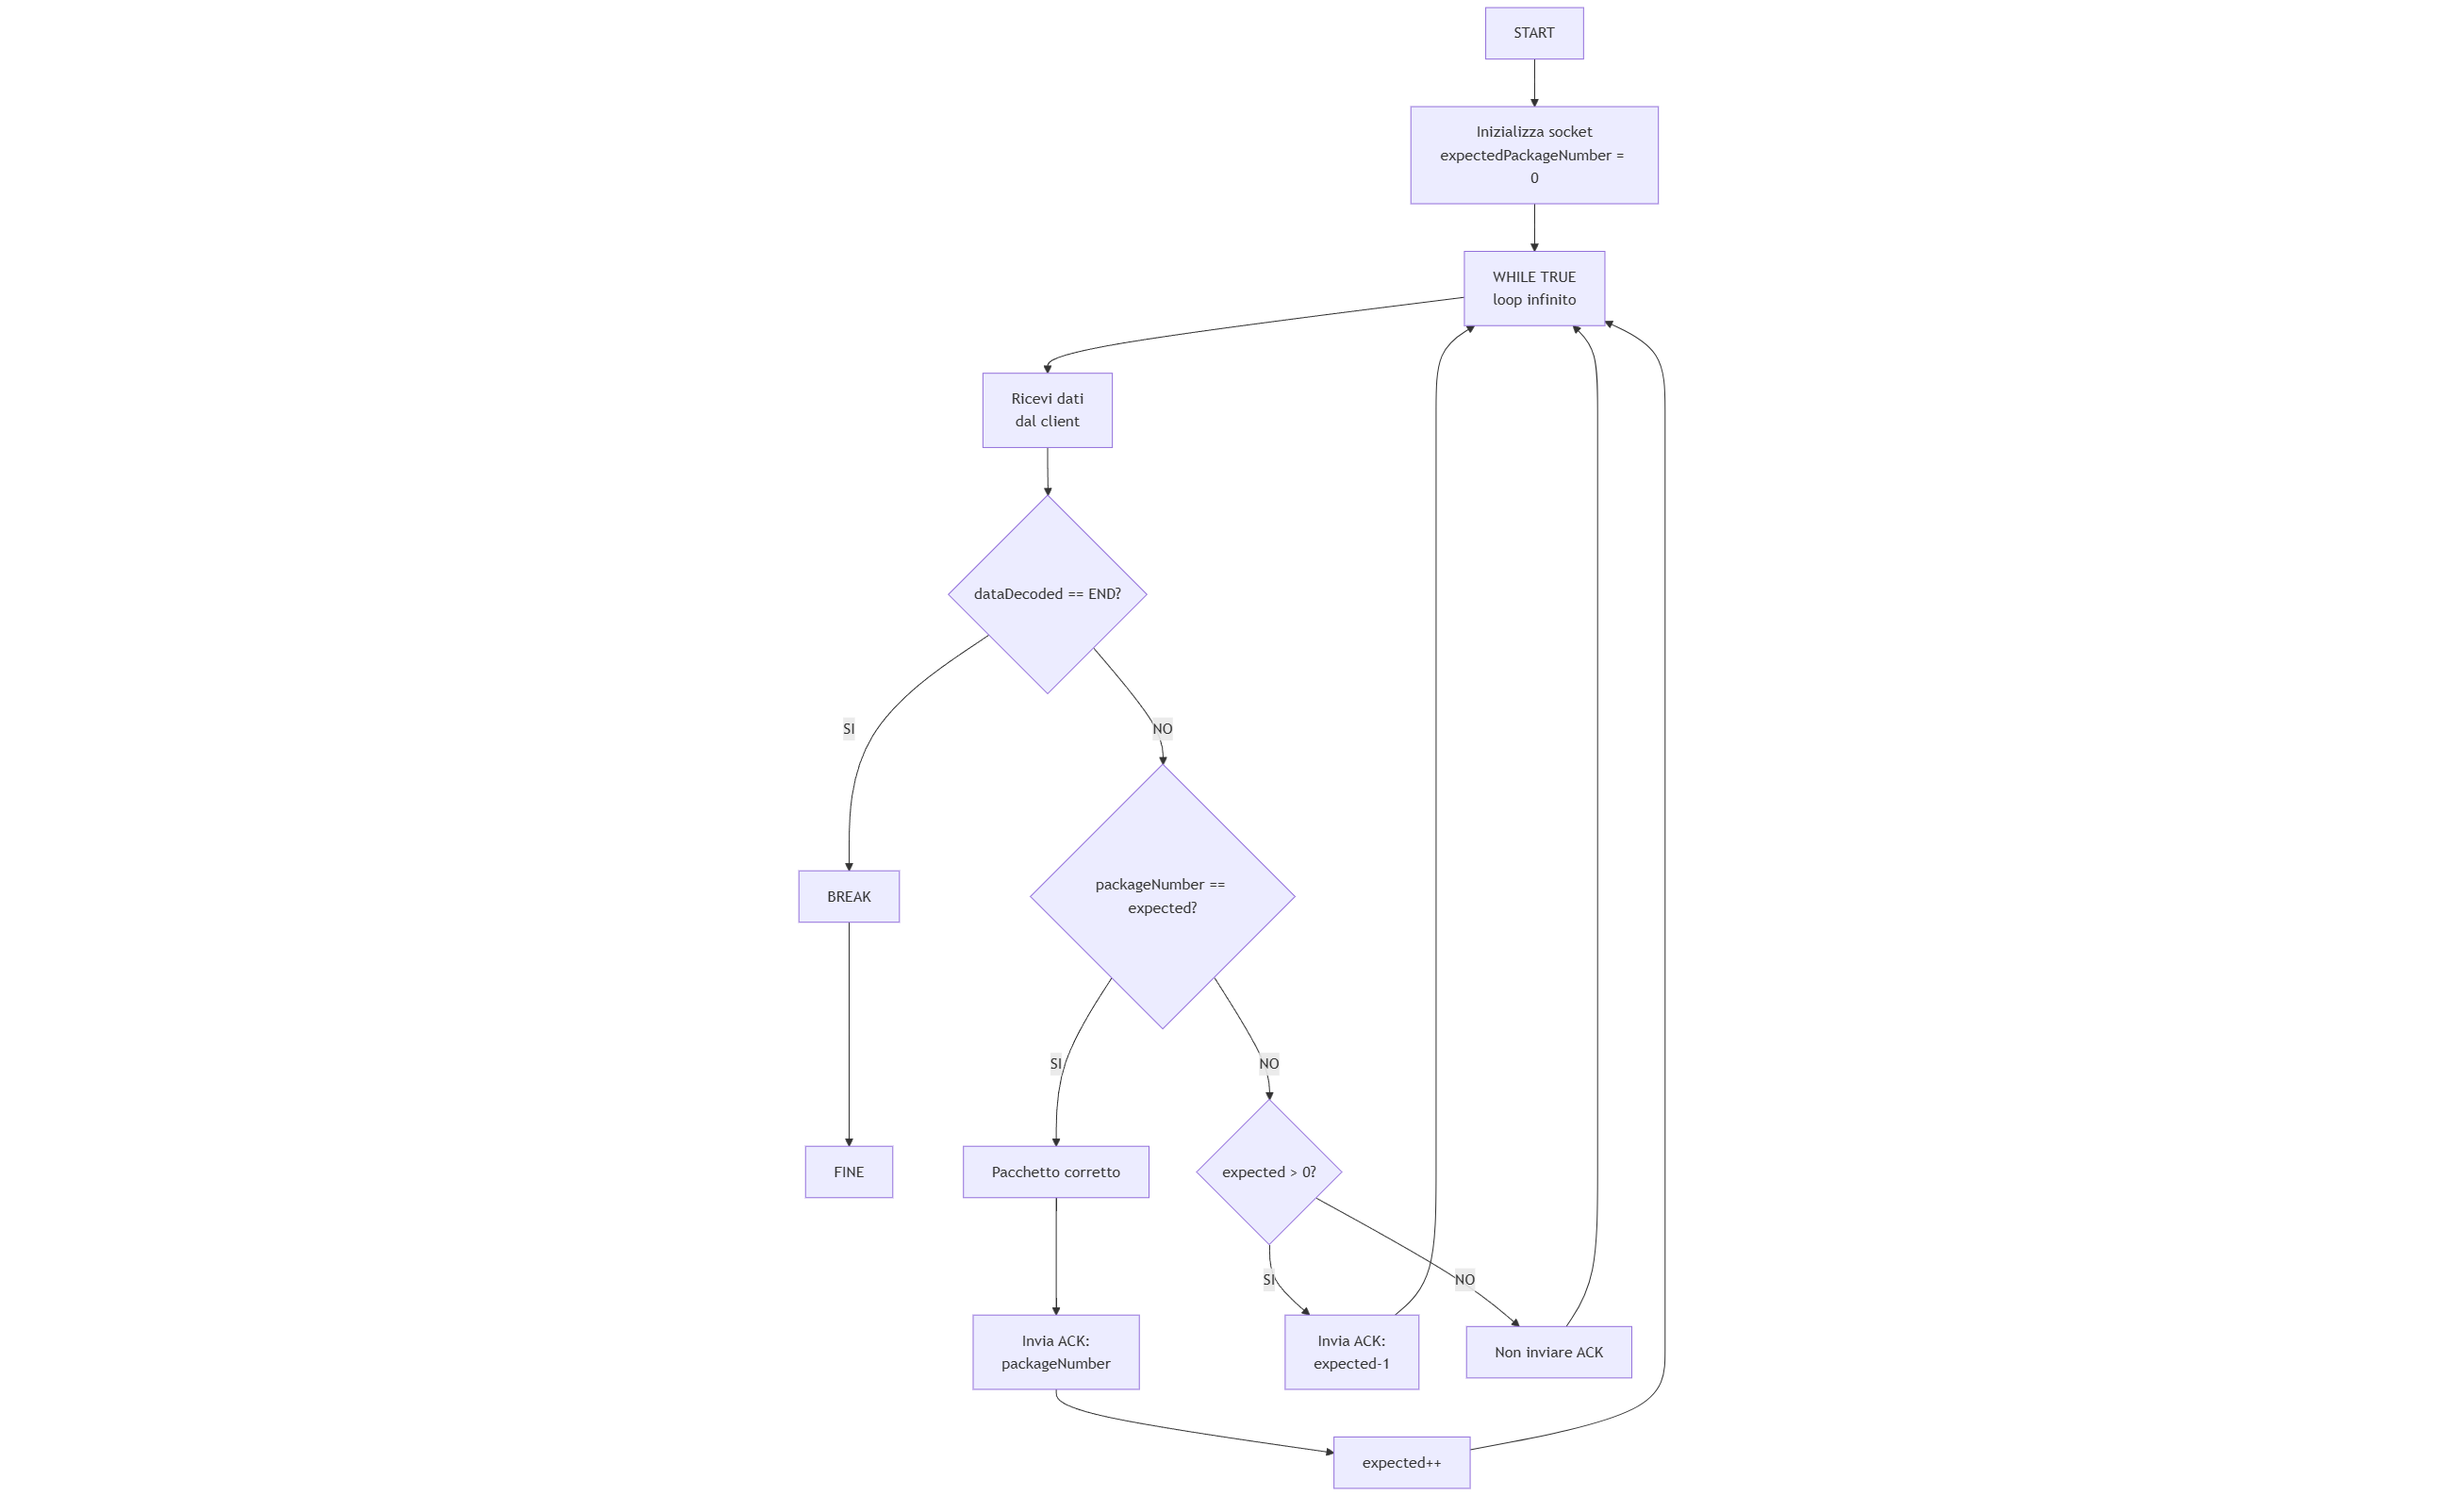
\includegraphics[width=\paperwidth, height=0.85\textheight, keepaspectratio]{img/SchemaDiFlussoServer.png}
    \caption{Schema di flusso del server}
    \label{img: schema di flusso del server}
\end{figure}
\section{Caratteristiche del Protocollo Go-Back-N}
\textbf{Vantaggi}
\begin{itemize}
    \item \textbf{Semplicità}: Il ricevitore mantiene solo il numero di sequenza atteso
    \item \textbf{Efficienza di memoria}: Buffering minimo nel ricevitore
    \item \textbf{Controllo di flusso}: La finestra scorrevole limita i pacchetti in volo
\end{itemize}
\textbf{Svantaggi}
\begin{itemize}
    \item \textbf{Ritrasmissioni ridondanti}: In caso di perdita, tutti i pacchetti successivi vengono ritrasmessi
    \item \textbf{Efficienza limitata}: Con alta perdita di pacchetti, le prestazioni degradano
\end{itemize}
\section{Gestione degli Errori}
\begin{itemize}
    \item \textbf{Perdita di pacchetti}: Simulata casualmente nel client.
    \item \textbf{Timeout}: Attivazione della ritrasmissione automatica
    \item \textbf{ACK duplicati}: Ignorati dal client se inferiori alla base della finestra
    \item \textbf{Pacchetti fuori ordine}: Scartati dal server con invio di ACK duplicato
\end{itemize}
\section{Metrice Monitorate}
\textbf{Client}
\begin{itemize}
    \item Pacchetti inviati
    \item ACK ricevuti
    \item Ritrasmissioni effettuate
    \item Perdite simulate
\end{itemize}
\textbf{Server}
\begin{itemize}
    \item Pacchetti ricevuti
    \item ACK inviati
    \item Pacchetti fuori ordine
\end{itemize}
\end{document}